In the previous section, we describe a general methodology for training Transformer models to in-context learn a class of functions.
Here, we focus on a simple function class---namely linear functions---and study how well models trained using our methodology can in-context learn this class.

\paragraph{Prompt distribution.}
We consider the class of linear functions $\mathcal{F} = \left\{f \mid  f(x) = w^\top x,\  w\in\mathbb{R}^d\right\}$, in $d$ dimensions where $d=20$.
We sample $x_1, \ldots, x_k$, $x_\text{query}$, and $w$ independently from the isotropic Gaussian distribution $N(0, I_d)$.
We then compute each $y_i=w^\top x_i$ and construct the prompt as $P = (x_1,\ y_1, \ x_2,\ y_2, \ldots,\ x_k,\ y_k,\ x_{\text{query}})$.

% Concretely, we will train a self-attention, decoder-only transformer, similar to the GPT2~\citep{gpt2} model family.
% The structure of this model allows us to efficiently obtain a prediction for each point in the sequence.
% We use a decoder-only auto-regressive transformer~\citep{}, as this ensures that the output of the model at point $i$ only depends on points less than that.
% We train the model on the average of the L2-squared loss which simultaneously supervises predictions at all prompt lengths.
% We also do curriculum.


\paragraph{Baselines.} To contextualize the performance of our trained model, we compare it to other learning algorithms: 
(a) the least squares estimator, computing the minimum-norm linear fit to the in-context examples $(x_i,\ y_i)$,
(b) $n$-Nearest Neighbors, averaging the $y_i$ values for the $n$ nearest neighbors of $x_{\text{query}}$,
(c) averaging the values $y_ix_i$ to estimate $w$ and compute the inner product of this estimate with $x_\text{query}$.
Least squares is the optimal estimator for this problem and thus serves as a lower bound to the best error one can achieve.
The other two baselines are consistent (but sub-optimal) estimators that are easier to compute and thus provide an estimate of the performance achieved by simple approaches.
See Appendix~\ref{app:baselines} for more details.

\subsection{Transformers can in-context learn linear functions}
\label{sec:linear_functions_1}
We show the in-context learning ability of the resulting model along with the relevant baselines in Figure \ref{fig:core}.
The trained Transformer is able to in-context learn the class of linear functions with respect to the prompt distribution specified above,
%\pl{'random' is a bit loose here...it might be useful to be precise about what function class we're in-context learning (hmm...technically we have to say we in-context learn the distribution over some class)}
performing comparably to the optimal least squares estimator for any number of in-context examples considered.
While the simpler baselines achieve non-trivial error, they are far worse, indicating that the trained model encodes a  more complex algorithm.

\begin{figure}[htp]
    \centering
    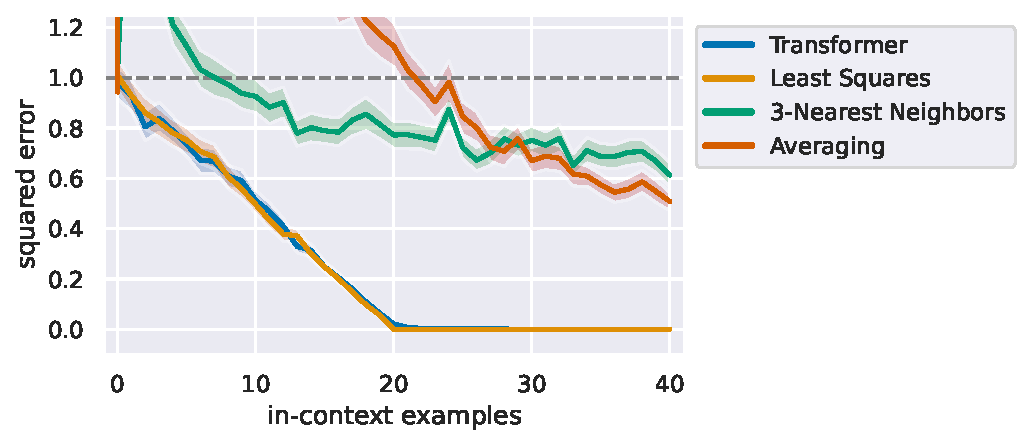
\includegraphics[width=.65\textwidth]{figures/core.pdf}
    %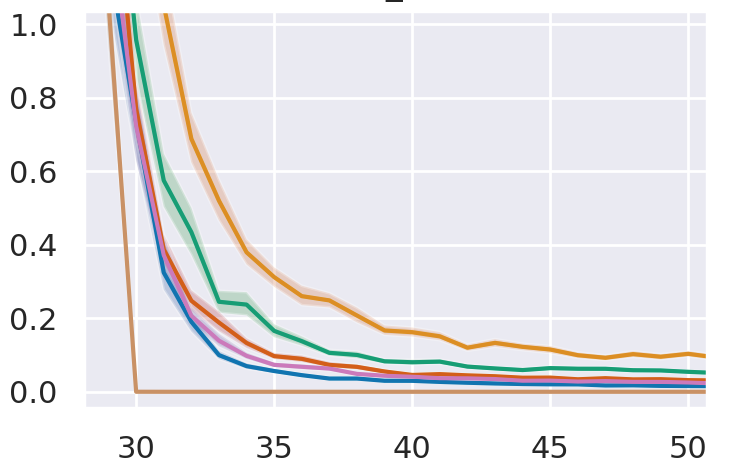
\includegraphics[width=.25\textwidth]{figures/zoom.png}
        \caption{
    \emph{Evaluating the trained Transformer on in-context learning linear functions.}
    We plot the normalized squared error of the Transformer $((M(P) - w^\top x_{\text{query}} )^2/d)$, along with the relevant baselines, as a function of the number of in-context examples.
    Transformer's error decreases at a rate comparable to least squares.
    When the number of in-context examples reaches the problem dimension $d$ (here 20), least squares achieves $0$ error while the Transformer achieves an error of $0.02$, improving to $0.0006$ at $2d$ in-context examples.
    While the simple baselines obtain better-than-trivial error (zero estimator, dashed line), their performance is relatively poor.
    (Error averaged over 1280 prompts. 90\% confidence intervals over 1000 bootstrap trials.)}
    \label{fig:core}
\end{figure}

\paragraph{Can memorization of training prompts explain model performance?} 
% \pl{and we've already shown that we have models that can in-context learn (in the distributional sense - might want to give a name for that); don't make it seem like that question is open; now state the next question more precisely: is the ability to in-context learn linear functions coming from the fact that the model was trained on those functions? 'generalizing or memorizing' seems a bit too loosey-goosey for my taste especially since we have the in-context and the meta levels to contend with
% }
%Is it possible that the model performs in-context learning by memorizing the prompts seen during training?
Note that the probability of the model encountering a training prompt similar to the one used for testing is astronomically low---the prompt inputs alone lie in a 800-dimensional space when predicting with $2d$ in-context examples ($d=20$).
Moreover, even considering the possibility that the model encountered a similar \emph{weight vector} during training cannot explain its performance.
That is, the model encounters 32 million random weight vectors during training and even using the best of these vectors would lead to an expected error of around $0.2$ (computed empirically, see Appendix \ref{app:memorization} for details).
 However, the model is able to achieve an error of less than $0.001$ for a prompt with $2d$ in-context examples. Further, in Section \ref{sec:factors}, we show that the model is able to obtain a similar error even when trained on prompts generated using only $10,000$  distinct weight vectors, in which case the best weight vector seen during training would yield an even worse error of around $0.5$. Thus, the model cannot be relying on memorization of training prompts or weight vectors, and instead encodes an algorithm capable of in-context learning linear functions that are very different from those seen during training.



\subsection{What functions is the model learning in-context?}
Recall that the goal of our model is: given the prompt $P=(x_1,\ w^\top x_1, \ldots, x_k,\ w^\top x_k,\ x_{\text{query}})$, output $w^\top x_\text{query}$.
Thus, if we fix the prefix given by the $k$ in-context examples, we can view the output of the model  as a function  $\hat{f}_{w,  x_{1:k}}(x_{\text{query}})$, that approximates $w^\top x_{\text{query}}$.
When $k < d$ (fewer in-context examples than dimensions), the ground truth cannot be recovered perfectly  and the ideal model should approximate $(\text{proj}_{x_{1:k}}(w))^\top x_{\text{query}}$, where $\text{proj}_{x_{1:k}}(w)$ is the projection of $w$ onto the subspace spanned by $x_1,\ldots,x_k$. Here, we will evaluate how accurately the model approximates this.

\paragraph{Visualizing along a random direction.}
For a randomly sampled fixed prefix, we visualize $\hat{f}_{w,  x_{1:k}}(x_{\text{query}})$  as we vary the query input along a random direction $x$ (Figure~\ref{fig:random_lines}).
That is, we pick a random unit vector $x$, and evaluate $\hat{f}_{w,  x_{1:k}}(\lambda x)$ as we vary  $\lambda$, the distance of the query input from origin. 
We observe that  $\hat{f}_{w,  x_{1:d}}(\lambda x)$ and $\hat{f}_{w,  x_{1:2d}}(\lambda x)$ closely match the ground truth  and $\hat{f}_{w,  x_{1:d/2}}(\lambda x)$ matches the projected ground truth, when the distance from origin is not too large compared to the norm of a typical randomly sampled input. In fact, in Appendix~\ref{app:query}, we show that the model is quite robust to scaling the query input:  the error doesn't increase much as we scale up the query input by a factor of up to 2, or scale down by a factor of up to 16, and degrades slowly after that.

\begin{figure}
    \centering
    \begin{subfigure}[b]{0.69\textwidth}
        \centering
        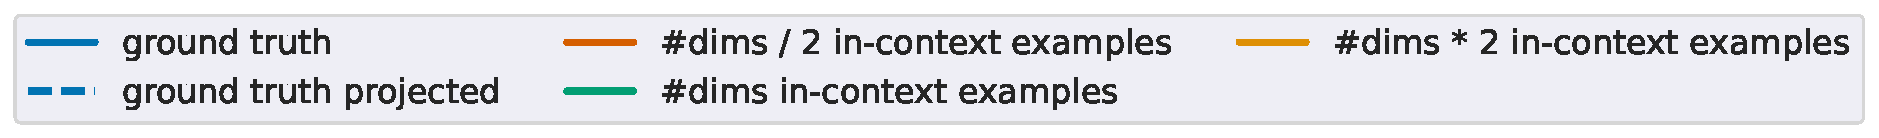
\includegraphics[width=.97\textwidth]{figures/visualizations/legend.pdf}
    
        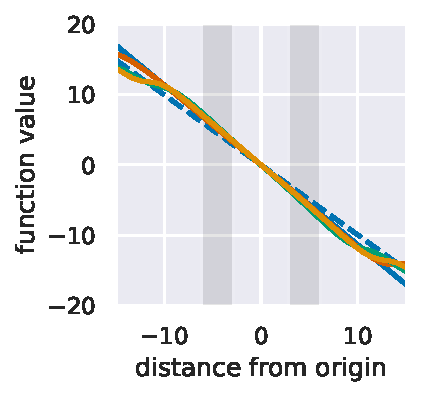
\includegraphics[height=0.3\textwidth]{figures/visualizations/vis_0.pdf}
        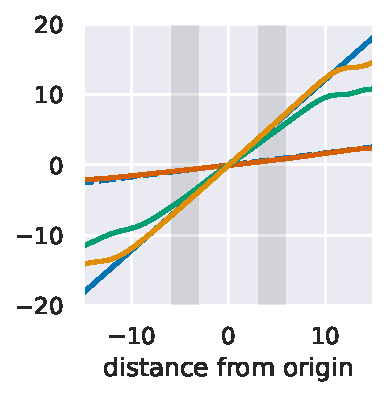
\includegraphics[height=0.3\textwidth]{figures/visualizations/vis_1.pdf}
        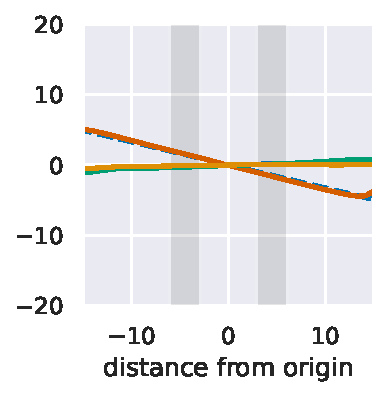
\includegraphics[height=0.3\textwidth]{figures/visualizations/vis_2.pdf}
        \caption{function visualizations}
        \label{fig:random_lines}
    \end{subfigure}
    \begin{subfigure}[b]{0.29\textwidth}
        \centering
        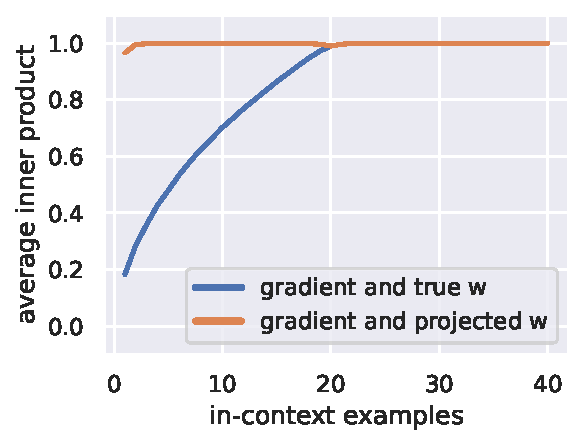
\includegraphics[width=\textwidth]{figures/gradients.pdf}
        \caption{gradients}
        \label{fig:gradients}
    \end{subfigure}

    \caption{\emph{Understanding the prefix-conditioned function}. 
    (a) We plot the model prediction as we fix the in-context examples and vary the query input along a random direction (for three random prompts).
    The shaded regions denote the intervals in which the norm of a randomly training input lies with probability 0.99. When the scale of the query input is close to this range, the model prediction is close to the ground truth linear function (or its projection to the space of in-context inputs when $k < d$).
    (b) We compute the gradient of the model prediction with respect to the query input, and plot its (normalized) inner product with the true $w$ and projected $w$, averaged over 1280 random prompts. The gradient aligns almost perfectly with $w$ when $k \geq d$, and with projected $w$ for all $k$, indicating that the model locally aligns with the ground truth.
    % The gradient is consistently quite close to the best $w$ estimate, indicating that the model is learning a locally correct function.
    }
    \label{fig:local}
\end{figure}


\paragraph{Local correctness.} 
So far, we have seen that the model is able to make predictions close to the ground truth for randomly drawn query inputs and in-context examples.
We will now turn our attention to the local change of $\hat f$ around $x_\text{query}$ by considering the gradient of the function $\hat{f}_{w,  x_{1:k}}(x_{\text{query}})$ with respect to $x_{\text{query}}$ (our model is fully differentiable so we can compute the gradient directly).
Since $\hat{f}$ computed by the model should ideally approximate $\text{proj}_{x_{1:k}}(w)^\top x$, this gradient should lie in the direction of the projected ground truth $\text{proj}_{x_{1:k}}(w)$.
In Figure~\ref{fig:gradients}, we show the inner product  between the gradient and $\text{proj}_{x_{1:k}}(w)$ (both normalized),  averaged over 1280 random prompts, and observe that they align almost perfectly. Since $\text{proj}_{x_{1:k}}(w) = w$ almost surely when $k \geq d$, we observe that the gradient also aligns with $w$ perfectly in this regime. Thus the model is locally correct with respect to changes in the query input.